% Chapter Template

\chapter{\textit{Behavior Trees} - Básicos} % Main chapter title

\label{Chapter2} % Change X to a consecutive number; for referencing this chapter elsewhere, use \ref{ChapterX}



\section{O que são \textit{Behavior Trees}?}
\textit{Behavior Trees}, ou BT, são estruturas que controlam a execução de um conjunto de ações por parte de um agente autónomo, de forma a descreverem o seu comportamento.
Este tipo de estrutura começou por ser utilizado especialmente em videojogos (para simular o comportamento de NPCs), mas com o passar do tempo áreas como a Robótica ou a Inteligência Artificial também o começaram a usar, devido à sua capacidade modular e reativa.

Formalmente, uma BT é uma árvore com raiz onde os nodos internos são chamados \textit{control flow nodes} e as folhas são chamadas de \textit{execution nodes}. Para cada nodo conetado usamos a terminologia de \textit{parent} (pai) e \textit{child} (filho).
A raiz é o único nodo que não tem pais, todos os outros nodos têm exatamente um pai.
Os \textit{control flow nodes} têm pelo menos um filho, já os \textit{execution nodes} não têm nenhum.

A figura \ref{fig:2.1} mostra um exemplo de uma BT, onde o nodo a verde é a raiz, os nodos a cinzento são \textit{control flow nodes} e os restantes são \textit{execution nodes}.

\begin{figure}[H]
\centering
\begin{behavior}
    [\rootnode
        [\sequence
            [\action{Walk to door}]
            [\selector
                [\action{Open door}]
                [\sequence
                    [\action{Unlock door}]
                    [\action{Open door}]
                ]
                [\action{Smash door}]
            ]
            [\action{Walk through door}]
            [\action{Close door}]
        ]
    ]
\end{behavior}
\caption{Exemplo de uma BT.}
\label{fig:2.1}
\end{figure}

\section{Execução}
Uma BT começa a sua execução pelo nodo raiz que gera sinais chamados \textit{ticks} com uma determinada frequência, que são enviados para os seus filhos.
Estes sinais permitem a execução dos nodos.

Qualquer nodo, não importa o tipo, ao ser executado retorna um de três estados: 
\begin{itemize}
    \item \textit{Success} - foi executado com sucesso;
    \item \textit{Failure} - não conseguiu ser executado;
    \item \textit{Running} - ainda está a executar.
\end{itemize}




\section{Nodos}

\subsection{\textit{Control Flow Nodes} - Clássicos}
\textit{Control flow nodes} são nodos estruturais, que não têm qualquer impacto no estado global do sistema.
Na formulação clássica, existem 4 categorias deste tipo de nodo: \textit{Sequence}, \textit{Selector (ou Fallback)}, \textit{Parallel} e \textit{Decorator}.

\paragraph{Sequence}{
    Um nodo \textit{Sequence} visita (envia \textit{ticks}) todos os filhos por ordem, começando pelo primeiro, e se este retornar \textit{Success}, chama o segundo, e por aí em diante.
    Caso um filho falhe, o nodo \textit{Sequence} retorna \textit{Failure} imediatamente.
    Caso todos os filhos sucedam, o nodo retorna \textit{Success}.
    Caso um filho retorne \textit{Running}, o nodo retorna também \textit{Running}.

    \begin{figure}[H]
    \centering
    \begin{behavior}
        [\sequence
            [\action{Child 1}]
            [\action{Child 2}]
            [{\textbf{. . .}}, inner sep=10pt]
            [\action{Child N}]
        ]
    \end{behavior}
    \caption{Estrutura de um nodo \textit{Sequence}.}
    \label{fig:2.2}
    \end{figure}
}

\paragraph{Selector}{
    Tal como o \textit{Sequence}, o nodo \textit{Selector} visita todos os filhos por ordem, mas só avança para o próximo se o filho que está a ser executado retorne \textit{Failure}.
    Caso um filho suceda, o nodo \textit{Sequence} retorna \textit{Sucess} imediatamente.
    Caso todos os filhos falhem, retorna \textit{Failure}.
    Caso um filho retorne \textit{Running}, o nodo retorna também \textit{Running}.

    \begin{figure}[H]
    \centering
    \begin{behavior}
        [\selector
            [\action{Child 1}]
            [\action{Child 2}]
            [{\textbf{. . .}}, inner sep=10pt]
            [\action{Child N}]
        ]
    \end{behavior}
    \caption{Estrutura de um nodo \textit{Selector}.}
    \label{fig:2.3}
    \end{figure}
}

\paragraph{Parallel}{
    Um nodo \textit{Parallel}, como o nome indica, visita todos os filhos paralelamente.
    Para $M \leq N$, retorna \textit{Success} caso $M$ filhos sucedam, e retorna \textit{Failure} caso $N - M + 1$ filhos retornem \textit{Failure}.
    Caso contrário, retorna \textit{Running}.

    \begin{figure}[H]
    \centering
    \begin{behavior}
        [\parallel{M}
            [\action{Child 1}]
            [\action{Child 2}]
            [{\textbf{. . .}}, inner sep=10pt]
            [\action{Child N}]
        ]
    \end{behavior}
    \caption{Estrutura de um nodo \textit{Parallel} com taxa de sucesso $M$.}
    \label{fig:2.4}
    \end{figure}
}

\paragraph{Decorator}
    Um nodo \textit{Decorator} tem um único filho, e utiliza uma política (conjunto de regras) definida pelo utilizador para manipular o estado de retorno desse filho ou controlar a sua execução.

    \begin{figure}[H]
    \centering
    \begin{behavior}
        [\decorator{$\delta$},
            [\action{Child}]
        ]
    \end{behavior}
    \caption{Estrutura de um nodo \textit{Decorator} com uma política $\delta$.}
    \label{fig:2.5}
    \end{figure}
    
    Exemplos de nodos \textit{Decorator}:
    \begin{itemize}
        \item \textit{inverter} - inverte o estado \textit{Success/Failure} retornado pelo filho;
        \item \textit{max-$N$-tries} - o filho só pode falhar $N$ vezes, depois retorna sempre \textit{Failure} sem enviar \textit{ticks} para o filho.
        \item \textit{max-$T$-seconds} - deixa o filho correr durante $T$ segundos. Se depois disto o filho retornar \textit{Running}, o nodo retorna \textit{Failure} sem correr o filho.
    \end{itemize}






\subsection{\textit{Execution Nodes}}
\textit{Execution nodes} são os nodos mais simples, porém os mais poderosos, pois contêm os testes ou ações que serão implementados pelo sistema.
Existem 2 categorias para este tipo de nodos: \textit{Action} e \textit{Condition}.

\paragraph{Action}{
    Quando recebe \textit{ticks}, um nodo \textit{Action} executa um ou mais comandos.
    Retorna \textit{Success} se a ação foi corretamente completada ou \textit{Failure} se a ação falhou.
    Enquanto está a ser executado, retorna \textit{Running}.

    \begin{figure}[H]
    \centering
    \begin{behavior}
        [\action{Action}]
    \end{behavior}
    \caption{Estrutura de um nodo \textit{Action}.}
    \label{fig:2.7}
    \end{figure}
}

\paragraph{Condition}{
    Quando recebe \textit{ticks}, um nodo \textit{Condition} verifica uma proposição.
    Retorna \textit{Success} ou \textit{Failure} dependendo se a proposição é válida ou não.
    De notar que um nodo \textit{Condition} nunca retorna um estado \textit{Running}.

    \begin{figure}[H]
    \centering
    \begin{behavior}
        [\condition{Condition}]
    \end{behavior}
    \caption{Estrutura de um nodo \textit{Condition}.}
    \label{fig:2.8}
    \end{figure}

    \hr
    \paragraph{\textit{NOTA:}}{
        \textit{
        Quando juntamos o nodo Condition com os nodos Sequence e Selector podemos criar uma expressão condicional (if-then-else). Vejamos o seguinte exemplo:
        }
        \begin{figure}[H]
        \centering
        \begin{behavior}
            [\selector
                [\sequence
                    [\condition{Shop is open}]
                    [\action{Go shopping}]
                ]
                [\action{Go home}]
            ]
        \end{behavior}
        \caption{Exemplo de uma expressão condicional numa BT.}
        \label{fig:2.9}
        \end{figure}

        \textit{
        Como podemos ver, a escolha da ação a executar alterna entre ir às compras ou ir embora consoante a loja esteja aberta ou não. Ou seja,
        }

        \begin{center}
            \textit{
            \underline{\textbf{if}} Shop is open \underline{\textbf{then}} Go shopping \underline{\textbf{else}} Go home
            }
        \end{center}
    }
    \hr
}



\subsection{\textit{Control Flow Nodes} - Novos}
Para além dos \textit{control flow nodes} existentes na formulação clássica das BTs, podemos ter outras categorias de nodos, de forma a proporcionar uma melhoria a tanto a nível de AI, como a nível de imprevisibilidade, ou até mesmo apenas algo que facilite a implementação de certos comportamentos por parte do programador.
Visto isto, decidimos introduzir um novo nodo: \textit{Probability Selector}.

\paragraph{Probability Selector}{
    
    Um nodo \textit{Probability Selector} pode ser visto como uma ``extensão'' ao nodo \textit{Selector}. 
    A única diferença é que, enquanto o \textit{Selector} clássico visita os filhos por ordem, este novo nodo executa-os de uma forma aleatória tendo em conta que cada filho tem uma certa probabilidade, definida pelo utilizador, de ser escolhido.

    \begin{figure}[H]
    \centering
    \begin{behavior}
        [\probselector
            [\action{Child 1}, edge label = {node [above, sloped] {$P_1$}}],
            [\action{Child 2}, edge label = {node [above, sloped] {$P_2$}}],
            [{\textbf{. . .}}, inner sep=10pt],
            [\action{Child N}, edge label = {node [above, sloped] {$P_N$}}]
        ]
    \end{behavior}
    \caption{Estrutura de um nodo \textit{Probability Selector}.}
    \label{fig:2.6}
    \end{figure}

    Com este novo nodo, conseguimos atingir um novo nível de AI, pois permite-nos construir comportamentos não só mais imprevisíveis, como também influenciados por fatores externos.
    Analisemos a seguinte situação:
    \\

    \textit{
        Num videojogo, o nosso herói quer convidar um certo NPC para o acompanhar numa missão muito perigosa.
        No entanto há um problema... o NPC é pouco corajoso.
    }
    \\

    Se olharmos para esta situação de forma racional, é óbvio que ele irá rejeitar este convite.
    Mas não existirá na mesma a possibilidade de ele por acaso aceitar?
    Vejamos o seguinte:
    \\

    \textit{
        Mas por obra do acaso o dia até está a correr bem ao NPC, e naquele momento ele sente-se confiante e, contra todas as espetativas, decide aceitar o convite.
    }
    \\

    Ok, temos aqui novas informações acerca do comportamento do NPC, mas nada demais.
    Construindo um \textit{if-then-else} com a nossa BT conseguimos resolver este problema.
    Se o NPC estiver confiante aceita, senão rejeita.

    Mas e se mesmo que esteja confiante, o medo leva a melhor e ele decide rejeitar?
    No mundo real, não conseguimos prever com 100\% de certeza o comportamento de uma certa pessoa.
    Existe aqui um nível de imprevisibilidade que não é atingível utilizando apenas os nodos clássicos das BT.

    Posto isto, vamos adicionar esta subárvore com o nosso novo nodo ao comportamento do NPC:

    \begin{figure}[H]
    \centering
        \begin{behavior}
            [\probselector
                [\action{Accept}, edge label = {node [midway, above, sloped] {$P_1$}}],
                [\action{Reject}, edge label = {node [midway, above, sloped] {$P_2$}}]
            ]
        \end{behavior}

        \begin{align*}
            P_1 &= \frac{C}{10} \\
            P_2 &= 1 - \frac{C}{10}
        \end{align*}
        onde $C \in [0,10]$ é um valor , criado pelo programador, que representa o nível de coragem do NPC.
    \end{figure}
    
    O que esta subárvore diz é que, mesmo que seja muito pouco provável (porque tem um $C$ reduzido), existe a possibilidade do NPC aceitar o convite, quer seja por estar confiante, ou por outra razão qualquer que não diz respeito ao jogador.

    Mesmo não sendo muito correto (porque não sabemos que fatores levam à existência desta possibilidade), é uma aproximação interessante à tal imprevisibilidade que existe na vida real, permitindo a criação de comportamentos ainda mais complexos.

}








\section{Exemplo - \textit{PACMAN}}

Para percebermos melhor as aplicações das BTs, decidimos escolher como exemplo aplicacional o jogo do PAC-MAN da \textit{Namco’s}. 

O jogo do PAC-MAN é um jogo \textit{single player}, em que se passsa num labirinto que vai mudando a medida que o jogador passa de nivel. O jogador controla um boneco chamado de PAC-MAN, que tem como objectivo comer comida no labirinto e fugir dos inimigos chamados de fantasmas. Esta comida será representada por uma bolinha, sendo que existem 2 tipos de comida, a comida "normal" é representada por uma bolinha mais pequena, sendo que a bolinha maior após ingerida torna os fantasmas vulneráveis podendo o jogador comer os fantasmas durante um determinado tempo, após esse tempo os fantasmas regressam ao seu estado inicial. Os fantasmas irão perseguir o jogador, sendo que o objectivo deste será fugir destes ou come-los caso estes estejam vulneráveis. Por fim o jogador transita para o proximo nivel assim que comer toda a comida existente no labirinto.

\begin{figure}[h!]
\centering
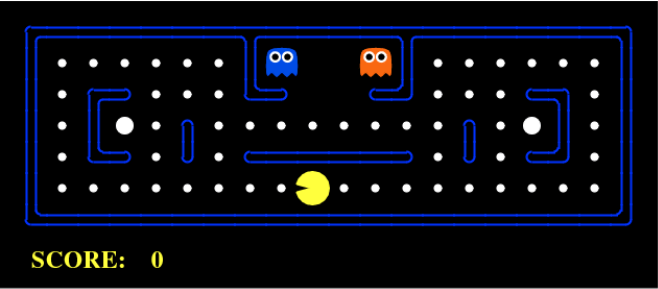
\includegraphics[scale=0.5]{Figures/PACMAN.PNG}
\caption{Exemplo do jogo de PAC-MAN}
\label{fig:traducao}
\end{figure}

Foi importante perceber como funciona o jogo numa fase inicial pois, para definirmos uma BT para o jogador precisamos de perceber qual o seu comportamento. Dito isso, percebemos que numa fase inicial o jogador deverá verificar se não se encontra nenhum fantasma perto, caso se encontre deverá fugir deste, caso estes se encontrem vulneráveis o jogador deverá come-los. Caso não se encontre nenhum fantasma por perto o jogador deverá comer a comida que se encontra no labirinto. Após a nálise do comportamento, iremos em seguida mostrar a respectiva BT.


        \begin{figure}[H]
        \centering
        \begin{behavior}
            [\selector
                [\sequence
                    [\condition{Fantasmas Perto}]
                    [\selector
                        [\sequence
                            [\condition{Fantasmas Vulneráveis}]
                            [\action{Perseguir Fantasmas}]
                        ]
                        [\action{Fugir dos Fantasmas}]
                    ]
                ]
                [\action{Comer a Comida}]
            ]
        \end{behavior}
        \caption{Exemplo da BT de um jogador de PAC-MAN.}
        \label{fig:2.9}
        \end{figure}